\documentclass[12pt,addpoints]{evalua}
\grado{4$^\circ$ de Primaria}
\cicloescolar{2024-2025}
\materia{Matemáticas}
\unidad{}
\title{Examen General}
\aprendizajes{\scriptsize
	  \item Expresa oralmente la sucesión numérica hasta cuatro cifras, en español y hasta donde sea posible, en su lengua materna, de manera ascendente y descendente a partir de un número natural dado; además, conoce los números romanos y su equivalencia en notación decimal.\\[-1.8em]
      \item Representa, con apoyo de material concreto y modelos gráficos, fracciones: medios, cuartos, octavos, dieciseisavos, para expresar el resultado de mediciones y repartos en situaciones vinculadas a su contexto.\\[-1.8em]
      \item Resuelve situaciones problemáticas vinculadas a su contexto que implican sumas o restas de números naturales de hasta cuatro cifras utilizando los algoritmos convencionales y números decimales hasta milésimos, con apoyo de material concreto y representaciones gráficas; además, que implican multiplicaciones de números naturales de hasta tres por dos cifras, a partir de diversas descomposiciones aditivas y el algoritmo convencional y el uso de un algoritmo para dividir números naturales de hasta tres cifras entre un número de una o dos cifras; reconoce al cociente y al residuo como resultado de una división.
	  }
\author{Prof.: Julio César Melchor Pinto}
\begin{document}
\tableofcontents
\newpage
\begin{questions}\large
	\addcontentsline{toc}{section}{Unidad 1}
	\section*{Unidad 1}
	\addcontentsline{toc}{subsection}{Escritura de cantidades}
	\subsection*{Escritura de cantidades}

	\question[2]{Escribe sore la línea los siguientes números:

		\begin{multicols}{2}
			\begin{parts}
				 %\part \fillin[  254][1.5cm] Doscientos cincuenta y cuatro.
				 %\part \fillin[  314][1.5cm] Trescientos catorce.
				\part \fillin[  431][1cm] Cuatrocientos treinta y uno.
				% \part \fillin[ 1024][1.5cm] Mil veinticuatro.s
				\part \fillin[ 1849][1cm] Mil ochocientos cuarenta y nueve.
				\part \fillin[14005][1cm] Catorce mil cinco.
				 \part \fillin[13990][1cm] Trece mil novecientos noventa.
				% \part \fillin[11300][1.5cm] Once mil trescientos.
				% \part \fillin[14400][1.5cm] Catorce mil cuatrocientos.
				% \part \fillin[15081][1.5cm] Quince mil ochenta y uno.
				 \part \fillin[19111][1cm] Diescinueve mil ciento once.
				\part \fillin[20422][1cm] Veinte mil cuatrocientos veintidos.
			\end{parts}
		\end{multicols}
	}

	\addcontentsline{toc}{subsection}{Números romanos}
	\subsection*{Números romanos}

	\question[2]{Escribe el valor de los siguientes números romanos

		\begin{multicols}{2}
			\begin{parts}
				\part \fillin[$16$][1cm] XVI
				 \part \fillin[$482$][1cm] CDLXXXII
				% \part \fillin[$18$][1cm] XVIII
				\part \fillin[$98$][1cm] XCVIII
				\part \fillin[$64$][1cm] LXIV
				\part \fillin[$199$][1cm] CXCIX
				% \part \fillin[$36$][1cm] XXXVI
				% \part \fillin[$42$][1cm] XLII
				% \part \fillin[$37$][1cm] XXXVII
				\part \fillin[$63$][1cm] LXIII
				% \part \fillin[$29$][1cm] XXIX
				% \part \fillin[$34$][1cm] XXXIV
			\end{parts}
		\end{multicols}
	}

	\question[2]{Escribe en números romanos los siguientes números

		\begin{multicols}{2}
			\begin{parts}
				 \part 28  \fillin[XXVIII][2.5cm]
				\part 46  \fillin[XLVI][2.5cm]
				% \part 38  \fillin[XXXVIII][2.5cm]
				\part 150 \fillin[CL][2.5cm]
				 \part 82  \fillin[LXXXII][2.5cm]
				\part 199 \fillin[CXCIX][2.5cm]
				% \part 98  \fillin[XCVIII][2.5cm]
				\part 482 \fillin[CDLXXXII][2.5cm]
				% \part 45  \fillin[XLV][2.5cm]
				 \part 94  \fillin[XCIV][2.5cm]
				% \part 308 \fillin[CCCVIII][2.5cm]
				 \part 40  \fillin[XL][2.5cm]
			\end{parts}
		\end{multicols}
	}

	\addcontentsline{toc}{subsection}{Sistema decimal}
	\subsection*{Sistema decimal}
	% \subsection*{\ifprintanswers{Posicionamiento decimal 1                      }\else{}\fi}
	% \subsection*{\ifprintanswers{Posicionamiento decimal 2                      }\else{}\fi}

	\question[2]{Señala la opción que responda correctamente a cada una de las siguientes preguntas:

		\begin{multicols}{2}
			\begin{parts}
				\part ¿Qué lugar ocupa el 6 en 6418?     \fillin[C][0.5cm]
				\part ¿Qué lugar ocupa el 2 en 206418?   \fillin[A][0.5cm]
				\part ¿Qué lugar ocupa el 2 en 87264?    \fillin[D][0.5cm]
				\part ¿Qué lugar ocupa el 1 en 1684?     \fillin[F][0.5cm]
				 \part ¿Qué lugar ocupa el 1 en 6138?     \fillin[D][0.5cm]
				 \part ¿Qué lugar ocupa el 8 en 198114?   \fillin[C][0.5cm]
				\part ¿Qué lugar ocupa el 7 en 46878?    \fillin[E][0.5cm]
				\part ¿Qué lugar ocupa el 4 en 149778?   \fillin[B][0.5cm]
			\end{parts}

			\columnbreak%

			\begin{choices}\Large
				\choice {\color{red}centenas de millar.}
				\choice {\color{blue}decenas de millar.}
				\choice {\color{Goldenrod}unidades de millar.}
				\choice {\color{red}centenas.}
				\choice {\color{blue}decenas.}
				\choice {\color{Goldenrod}unidades.}
			\end{choices}
		\end{multicols}
	}

% \subsection*{\ifprintanswers{Notación desarrollada 1                        }\else{}\fi}
	% \subsection*{\ifprintanswers{Notación desarrollada 2                        }\else{}\fi}
	\question[4]{Escribe la notación desarrollada de cada uno de los siguientes números:

		\begin{multicols}{2}
			\begin{parts}
				 \part $818 =$ \fillin[$800+10+8$][2.4in]
				\part $936 =$ \fillin[$900+30+6$][2.4in]
				 \part $4936 =$ \fillin[$4000+900+30+6$][2.4in]
				 \part $2096=$ \fillin[$2000+90+6$][2.4in]
				\part $4818 =$ \fillin[$4000+800+10+8$][2.4in]
				 \part $7145 =$ \fillin[$7000+100+40+5$][2.4in]
				\part $19679=$ \fillin[$10000+9000+600+70+9$][2.4in]
				\part $26324=$ \fillin[$20000+6000+300+20+4$][2.4in]
			\end{parts}
		\end{multicols}
	}

% \newpage
	% \subsection*{\ifprintanswers{Posicionamiento decimal y Notación desarrollada}\else{}\fi}

	\question[2]{Señala la opción que responda correctamente a cada una de las siguientes preguntas:

		\begin{multicols}{2}
			\begin{parts}
				\part En el número 3658, ¿qué número ocupa la posición de las decenas?

				\begin{oneparcheckboxes}
					\choice 3 \CorrectChoice 5 \choice 6 \choice 8 \choice 9
				\end{oneparcheckboxes}

				\part En el número 17542, ¿qué número ocupa la posición de las unidades de millar?

				\begin{oneparcheckboxes}
					\choice 1 \CorrectChoice 7 \choice 5 \choice 4 \choice 2
				\end{oneparcheckboxes}

				\part En el número 5984, ¿qué número ocupa la posición de las centenas?

				\begin{oneparcheckboxes}
					\choice 4 \choice 2 \choice 5 \choice 8 \CorrectChoice 9
				\end{oneparcheckboxes}

				\part En el número 7841, ¿qué número ocupa la posición de las decenas?

				\begin{oneparcheckboxes}
					\choice 1 \choice 7 \choice 8 \CorrectChoice 4 \choice 2
				\end{oneparcheckboxes}

				\part En el número 3918, ¿qué número ocupa la posición de las centenas?

				\begin{oneparcheckboxes}
					\choice 3 \choice 1 \choice 6 \choice 8 \CorrectChoice 9
				\end{oneparcheckboxes}

				% \part En el número 3621, ¿qué número ocupa la posición de las decenas?

				% \begin{oneparcheckboxes}
				% 	\CorrectChoice 2 \choice 3 \choice 6 \choice 8 \choice 1
				% \end{oneparcheckboxes}

				\part En el número 51362, ¿qué número ocupa la posición de las decenas de millar?

				\begin{oneparcheckboxes}
					\choice 3 \CorrectChoice 5 \choice 6 \choice 1 \choice 2
				\end{oneparcheckboxes}

				\part En el número 7584, ¿qué número ocupa la posición de las decenas?

				\begin{oneparcheckboxes}
					\choice 3 \choice 5 \choice 7 \CorrectChoice 8 \choice 4
				\end{oneparcheckboxes}

				\part En el número 9654, ¿qué número ocupa la posición de las centenas?

				\begin{oneparcheckboxes}
					\choice 3 \choice 5 \CorrectChoice 6 \choice 4 \choice 9
				\end{oneparcheckboxes}

				% \part En el número 240679, ¿qué número ocupa la posición de las centenas de millar?

				% \begin{oneparcheckboxes}
				% 	\choice 0 \choice 6 \CorrectChoice 2 \choice 7 \choice 9 \choice 4
				% \end{oneparcheckboxes}
				% \part En el número 41589, ¿qué número ocupa la posición de las decenas de millar?
				% \part En el número 8459, ¿qué número ocupa la posición de las centenas?
				% \part En el número 10562, ¿qué número ocupa la posición de las centenas?
				% \part En el número 24781, ¿qué número ocupa la posición de las decenas de millar?
				% \part En el número 7856, ¿qué número ocupa la posición de las decenas?
			\end{parts}
		\end{multicols}
	}

	\addcontentsline{toc}{subsection}{Números decimales}
	\subsection*{Números decimales}

	\question[4]{Escribe los siguientes números

		\begin{multicols}{2}
			\begin{parts}
				\part Seis enteros ciento veintiocho milésimas          \\ \hfill \fillin[$6.128$][1cm]
				 \part Catorce enteros veintinueve centésimas            \\ \hfill \fillin[$14.29$][1cm]
				 \part Cuarenta enteros dos décimas                      \\ \hfill \fillin[$40.2$][1cm]
				\part Tres enteros cincuenta y ocho centésimas          \\ \hfill \fillin[$3.58$][1cm]
				 \part Cuatro enteros sesenta y nueve milésimas          \\ \hfill \fillin[$4.069$][1cm]
				% \part Siete enteros cuatro décimas                      \\ \hfill \fillin[$ 7.4$][1cm]
				\part Dos enteros siete décimas                         \\ \hfill \fillin[$2.7$][1cm]
				\part Cuatro enteros ocho milésimas                     \\ \hfill \fillin[$4.008$][1cm]
				\part Siete enteros setenta y siete centésimas          \\ \hfill \fillin[$7.77$][1cm]
				\part Once enteros ochenta y nueve centésimas           \\ \hfill \fillin[$11.89$][1cm]
				% \part Treinta y ocho enteros nueve décimas              \\ \hfill \fillin[$38.9$][1cm]
				\part Veinticinco enteros ocho décimas                  \\ \hfill \fillin[$25.8$][1cm]
			\end{parts}
		\end{multicols}
	}

	\newpage

	\question[2]{Señala la opción que responda correctamente a cada una de las siguientes preguntas:

		\begin{multicols}{2}
			\begin{parts}
				\part En el número 1.829, ¿qué número ocupa la posición de las centésimas?

				\begin{oneparcheckboxes}
					\choice 1 \CorrectChoice 2 \choice 6 \choice 8 \choice 9
				\end{oneparcheckboxes}

				\part En el número 2.087, ¿qué número ocupa la posición de las décimas?

				\begin{oneparcheckboxes}
					\CorrectChoice 0 \choice 2 \choice 7 \choice 8 \choice 9
				\end{oneparcheckboxes}

				\part En el número 5.928, ¿qué número ocupa la posición de las décimas?

				\begin{oneparcheckboxes}
					\choice 5 \choice 2 \choice 6 \choice 8 \CorrectChoice 9
				\end{oneparcheckboxes}

				\part En el número 3.284, ¿qué número ocupa la posición de las milésimas?

				\begin{oneparcheckboxes}
					\choice 2 \choice 3 \CorrectChoice 4  \choice 8 \choice 9
				\end{oneparcheckboxes}

				\part En el número 1.285, ¿qué número ocupa la posición de las décimas?

				\begin{oneparcheckboxes}
					\choice 1 \CorrectChoice 2 \choice 5 \choice 8 \choice 9
				\end{oneparcheckboxes}

				\part En el número 1.823, ¿qué número ocupa la posición de las milésimas?

				\begin{oneparcheckboxes}
					\choice 1 \choice 2 \CorrectChoice 3 \choice 6 \choice 8
				\end{oneparcheckboxes}
			\end{parts}
		\end{multicols}
	}
	
	% \subsection*{\ifprintanswers{Suma de decimales            }\else{}\fi}
	\question[4]{Realiza las siguientes sumas con números decimales:

		\begin{multicols}{3}
			\begin{parts}
				\part \ifprintanswers{   \opadd[hfactor=decimal,resultstyle=\color{red},carryadd=true,carrysub=false]{4.9}{2.5} }
				\else{            \opadd[hfactor=decimal,resultstyle=\color{white},carryadd=false,carrysub=false]{4.9}{2.5}}
				\fi\\[2em]

				\part \ifprintanswers{   \opadd[hfactor=decimal,resultstyle=\color{red},carryadd=true,carrysub=false]{2.8}{3.1} }
				\else{           \opadd[hfactor=decimal,resultstyle=\color{white},carryadd=false,carrysub=false]{2.8}{3.1} }
				\fi\\[2em]

				\part \ifprintanswers{   \opadd[hfactor=decimal,resultstyle=\color{red},carryadd=true,carrysub=false]{3.19}{1.57} }
				\else{            \opadd[hfactor=decimal,resultstyle=\color{white},carryadd=false,carrysub=false]{3.19}{1.57} }
				\fi\\[2em]

				\part \ifprintanswers{   \opadd[hfactor=decimal,resultstyle=\color{red},carryadd=true,carrysub=false]{4.24}{2.33} }
				\else{            \opadd[hfactor=decimal,resultstyle=\color{white},carryadd=false,carrysub=false]{4.24}{2.33} }
				\fi\\[2em]

				\part \ifprintanswers{   \opadd[hfactor=decimal,resultstyle=\color{red},carryadd=true,carrysub=false]{2.928}{1.714} }
				\else{            \opadd[hfactor=decimal,resultstyle=\color{white},carryadd=false,carrysub=false]{2.928}{1.714} }
				\fi\\[2em]

				\part \ifprintanswers{   \opadd[hfactor=decimal,resultstyle=\color{red},carryadd=true,carrysub=false]{5.345}{2.514} }
				\else{           \opadd[hfactor=decimal,resultstyle=\color{white},carryadd=false,carrysub=false]{5.345}{2.514} }
				\fi\\[2em]
			\end{parts}
		\end{multicols}
	}

	% \subsection*{\ifprintanswers{Resta de decimales           }\else{}\fi}

	\question[4]{Realiza las siguientes restas con números decimales:

		\begin{multicols}{3}
			\begin{parts}
				\part \ifprintanswers{   \opsub[hfactor=decimal,resultstyle=\color{red},carryadd=true,carrysub=true]{4.3}{2.4} }
				\else{            \opsub[hfactor=decimal,resultstyle=\color{white},carryadd=false,carrysub=false]{4.3}{2.4} }
				\fi\\[2em]

				\part \ifprintanswers{   \opsub[hfactor=decimal,resultstyle=\color{red},carryadd=true,carrysub=true]{4.33}{2.47} }
				\else{            \opsub[hfactor=decimal,resultstyle=\color{white},carryadd=false,carrysub=false]{4.33}{2.47} }
				\fi\\[2em]

				\part \ifprintanswers{   \opsub[hfactor=decimal,resultstyle=\color{red},carryadd=true,carrysub=true]{5.81}{5.23} }
				\else{            \opsub[hfactor=decimal,resultstyle=\color{white},carryadd=false,carrysub=false]{5.81}{5.23} }
				\fi\\[2em]

				\part \ifprintanswers{   \opsub[hfactor=decimal,resultstyle=\color{red},carryadd=true,carrysub=true]{4.28}{1.96} }
				\else{            \opsub[hfactor=decimal,resultstyle=\color{white},carryadd=false,carrysub=false]{4.28}{1.96} }
				\fi\\[2em]

				\part \ifprintanswers{   \opsub[hfactor=decimal,resultstyle=\color{red},carryadd=true,carrysub=true]{3.14}{2.47} }
				\else{            \opsub[hfactor=decimal,resultstyle=\color{white},carryadd=false,carrysub=false]{3.14}{2.47} }
				\fi\\[2em]

				\part \ifprintanswers{   \opsub[hfactor=decimal,resultstyle=\color{red},carryadd=true,carrysub=true]{7.24}{3.58} }
				\else{            \opsub[hfactor=decimal,resultstyle=\color{white},carryadd=false,carrysub=false]{7.24}{3.58} }
				\fi\\[2em]
			\end{parts}
		\end{multicols}
	}
	\newpage
	\addcontentsline{toc}{section}{Unidad 2}
	\section*{Unidad 2}

	\addcontentsline{toc}{subsection}{Sumas}
	\subsection*{Sumas}

	\question[4]{Realiza las siguientes sumas:

		\begin{multicols}{4}
			\begin{parts}
				\part
				\ifprintanswers{\opadd[hfactor=decimal,resultstyle=\color{red},carryadd=true]{17}{18}}
				\else{\opadd[hfactor=decimal,resultstyle=\color{white},carryadd=false]{17}{18}}\fi\\[2em]

				\part
				\ifprintanswers{\opadd[hfactor=decimal,resultstyle=\color{red},carryadd=true]{1155}{893}}
				\else{\opadd[hfactor=decimal,resultstyle=\color{white},carryadd=false]{1155}{893}}\fi\\[2em]

				\part
				\ifprintanswers{\opadd[hfactor=decimal,resultstyle=\color{red},carryadd=true]{26}{19}}
				\else{\opadd[hfactor=decimal,resultstyle=\color{white},carryadd=false]{26}{19}}\fi\\[2em]

				\part
				\ifprintanswers{\opadd[hfactor=decimal,resultstyle=\color{red},carryadd=true]{2271}{1028}}
				\else{\opadd[hfactor=decimal,resultstyle=\color{white},carryadd=false]{2271}{1028}}\fi\\[2em]
				\part
				\ifprintanswers{\opadd[hfactor=decimal,resultstyle=\color{red},carryadd=true]{182}{149}}
				\else{\opadd[hfactor=decimal,resultstyle=\color{white},carryadd=false]{182}{149}}\fi\\[2em]

				\part
				\ifprintanswers{\opadd[hfactor=decimal,resultstyle=\color{red},carryadd=true]{73449}{358}}
				\else{\opadd[hfactor=decimal,resultstyle=\color{white},carryadd=false]{7449}{3258}}\fi\\[2em]

				\part
				\ifprintanswers{\opadd[hfactor=decimal,resultstyle=\color{red},carryadd=true]{482}{398}}
				\else{\opadd[hfactor=decimal,resultstyle=\color{white},carryadd=false]{482}{398}}\fi\\[2em]

				\part
				\ifprintanswers{\opadd[hfactor=decimal,resultstyle=\color{red},carryadd=true]{3234}{24156}}
				\else{\opadd[hfactor=decimal,resultstyle=\color{white},carryadd=false]{3234}{24156}}\fi\\[2em]

				% \part
				% \ifprintanswers{\opadd[hfactor=decimal,resultstyle=\color{red},carryadd=true]{37}{28}}
				% \else{\opadd[hfactor=decimal,resultstyle=\color{white},carryadd=false]{37}{28}}\fi
			\end{parts}
		\end{multicols}
	}

	\addcontentsline{toc}{subsection}{Restas}
	\subsection*{Restas}

	\question[4]{Realiza las siguientes restas:

		\begin{multicols}{4}
			\begin{parts}
				\part \ifprintanswers{   \opsub[hfactor=decimal,resultstyle=\color{red},carryadd=true,carrysub=true]{706}{589} }
				\else{            \opsub[hfactor=decimal,resultstyle=\color{white},carryadd=false,carrysub=false]{706}{589} }
				\fi\\[2em]

				\part \ifprintanswers{   \opsub[hfactor=decimal,resultstyle=\color{red},carryadd=true,carrysub=true]{3004}{1242} }
				\else{            \opsub[hfactor=decimal,resultstyle=\color{white},carryadd=false,carrysub=false]{3004}{1242} }
				\fi\\[2em]

				\part \ifprintanswers{   \opsub[hfactor=decimal,resultstyle=\color{red},carryadd=true,carrysub=true]{1600}{669} }
				\else{            \opsub[hfactor=decimal,resultstyle=\color{white},carryadd=false,carrysub=false]{1600}{669} }
				\fi\\[2em]

				\part \ifprintanswers{   \opsub[hfactor=decimal,resultstyle=\color{red},carryadd=true,carrysub=true]{4005}{2831} }
				\else{            \opsub[hfactor=decimal,resultstyle=\color{white},carryadd=false,carrysub=false]{4005}{2831} }
				\fi\\[2em]

				\part \ifprintanswers{   \opsub[hfactor=decimal,resultstyle=\color{red},carryadd=true,carrysub=true]{1200}{966} }
				\else{            \opsub[hfactor=decimal,resultstyle=\color{white},carryadd=false,carrysub=false]{1200}{966} }
				\fi\\[2em]

				\part \ifprintanswers{   \opsub[hfactor=decimal,resultstyle=\color{red},carryadd=true,carrysub=true]{42784}{34180} }
				\else{            \opsub[hfactor=decimal,resultstyle=\color{white},carryadd=false,carrysub=false]{42784}{34180} }
				\fi\\[2em]

				\part \ifprintanswers{   \opsub[hfactor=decimal,resultstyle=\color{red},carryadd=true,carrysub=true]{800}{744} }
				\else{            \opsub[hfactor=decimal,resultstyle=\color{white},carryadd=false,carrysub=false]{800}{744} }
				\fi\\[2em]

				\part \ifprintanswers{   \opsub[hfactor=decimal,resultstyle=\color{red},carryadd=true,carrysub=true]{37881}{24049} }
				\else{            \opsub[hfactor=decimal,resultstyle=\color{white},carryadd=false,carrysub=false]{37881}{24049} }
				\fi\\[2em]
				% \part \ifprintanswers{   \opsub[hfactor=decimal,resultstyle=\color{red},carryadd=true,carrysub=false]{2400}{211} }
				% \else{            \opsub[hfactor=decimal,resultstyle=\color{white},carryadd=false,carrysub=false]{2400}{211} }
				% \fi
				% \part \ifprintanswers{   \opsub[hfactor=decimal,resultstyle=\color{red},carryadd=true,carrysub=false]{1500}{1044} }
				% \else{            \opsub[hfactor=decimal,resultstyle=\color{white},carryadd=false,carrysub=false]{1500}{1044} }
				% \fi
				% \part \ifprintanswers{   \opsub[hfactor=decimal,resultstyle=\color{red},carryadd=true,carrysub=false]{2000}{1105} }
				% \else{            \opsub[hfactor=decimal,resultstyle=\color{white},carryadd=false,carrysub=false]{2000}{1105} }
				% \fi
				% \part \ifprintanswers{   \opsub[hfactor=decimal,resultstyle=\color{red},carryadd=true,carrysub=false]{1600}{669} }
				% \else{            \opsub[hfactor=decimal,resultstyle=\color{white},carryadd=false,carrysub=false]{1600}{669} }
				% \fi
			\end{parts}
		\end{multicols}
	}

	\addcontentsline{toc}{subsection}{Tablas de multiplicar}
	\subsection*{Tablas de multiplicar}

	\question[6]{Completa los espacios de acuerdo con las tablas de multiplicar:

		\begin{multicols}{4}
			\begin{parts}%\Large
				\part $7 \times 5=$ \fillin[35][0.5cm] \\
				\part $3 \times 6=$ \fillin[18][0.5cm] \\
				\part $9 \times \fillin[8][0.5cm]= 72$ \\
				\part $\fillin[6][0.5cm] \times 6= 36$ \\
				\part $\fillin[7][0.5cm] \times 8= 56$ \\
				\part $2 \times 9=$ \fillin[18][0.5cm] \\
				\part $4 \times \fillin[9][0.5cm]= 36$ \\
				\part $6 \times \fillin[7][0.5cm]= 42$ \\
				\part $9 \times 7=$ \fillin[63][0.5cm] \\
				\part $2 \times 7=$ \fillin[14][0.5cm] \\
				\part $\fillin[8][0.5cm] \times 3= 24$ \\
				\part $6 \times 9=$ \fillin[54][0.5cm] \\
			\end{parts}
		\end{multicols}
	}

	\newpage
	\addcontentsline{toc}{subsection}{Multiplicaciones}
	\subsection*{Multiplicaciones}

	\question[4]{Realiza las siguientes multiplicaciones:

		\begin{multicols}{3}
			\begin{parts}
				\part \ifprintanswers{   \opmul[hfactor=decimal,resultstyle=\color{red},displayintermediary=None]{314}{2} }
				\else{            \opmul[hfactor=decimal,resultstyle=\color{white},displayintermediary=None]{314}{2} }
				\fi\\[2em]

				\part \ifprintanswers{   \opmul[hfactor=decimal,resultstyle=\color{red},displayintermediary=None]{283}{44} }
				\else{            \opmul[hfactor=decimal,resultstyle=\color{white},displayintermediary=None]{283}{44} }
				\fi\\[2em]

				\part \ifprintanswers{   \opmul[hfactor=decimal,resultstyle=\color{red},displayintermediary=None]{2781}{5} }
				\else{            \opmul[hfactor=decimal,resultstyle=\color{white},displayintermediary=None]{2781}{5} }
				\fi\\[2em]

				\part \ifprintanswers{   \opmul[hfactor=decimal,resultstyle=\color{red},displayintermediary=None]{3914}{106} }
				\else{            \opmul[hfactor=decimal,resultstyle=\color{white},displayintermediary=None]{3914}{106} }
				\fi\\[2em]

				\part \ifprintanswers{   \opmul[hfactor=decimal,resultstyle=\color{red},displayintermediary=None]{255}{24} }
				\else{            \opmul[hfactor=decimal,resultstyle=\color{white},displayintermediary=None]{255}{24} }
				\fi\\[2em]

				\part \ifprintanswers{   \opmul[hfactor=decimal,resultstyle=\color{red},displayintermediary=None]{3533}{29} }
				\else{            \opmul[hfactor=decimal,resultstyle=\color{white},displayintermediary=None]{3533}{29} }
				\fi\\[2em]
			\end{parts}
		\end{multicols}
	}

	\addcontentsline{toc}{subsection}{Divisiones}
	\subsection*{Divisiones}
	\question[4]{Realiza las siguientes divisiones:

		\begin{multicols}{2}
			\begin{parts}
				\part \ifprintanswers{\large\opidiv{23}{6}} \\[2em]
				\else{           $6 \overline{) \ 23\ }$} \\[2em]
				\fi

				\part \ifprintanswers{\large\opidiv{200}{3}} \\[2em]
				\else{           $3 \overline{) \ 200\ }$} \\[2em]
				\fi

				\part \ifprintanswers{\large\opidiv{99}{8}} \\[2em]
				\else{           $8 \overline{) \ 99\ }$} \\[2em]
				\fi

				\part \ifprintanswers{\large\opidiv{283}{6}} \\[2em]
				\else{           $6 \overline{) \ 283\ }$} \\[2em]
				\fi

				\part \ifprintanswers{\large\opidiv{4032}{8}} \\[2em]
				\else{           $8 \overline{) \ 4032\ }$} \\[2em]
				\fi

				\part \ifprintanswers{\large\opidiv{644}{8}} \\[2em]
				\else{           $8 \overline{) \ 644\ }$} \\[2em]
				\fi

				\part \ifprintanswers{\large\opidiv{656}{7}} \\[2em]
				\else{           $7 \overline{) \ 656\ }$} \\[2em]
				\fi

				\part \ifprintanswers{\large\opidiv{2303}{7}} \\[2em]
				\else{           $7 \overline{) \ 2303\ }$} \\[2em]
				\fi
			\end{parts}
		\end{multicols}
	}

	\newpage
	\addcontentsline{toc}{section}{Unidad 3}
	\section*{Unidad 3}
	\addcontentsline{toc}{subsection}{Introducción a fracciones}
	\subsection*{Introducción a fracciones}

	\question[4]{Clasifica las siguientes fracciones en propias, impropias o mixtas:

		\begin{multicols}{4}
			\begin{parts}
				\part $\dfrac{5}{6}$   \fillin[Propia][0.75in]   \\[1em]
				\part $5\dfrac{5}{11}$ \fillin[Mixta][0.75in]    \\[1em]
				 \part $\dfrac{9}{7}$   \fillin[Impropia][0.75in] \\[1em]
				 \part $\dfrac{13}{14}$   \fillin[Propia][0.75in]   \\[1em]
				\part $1\dfrac{2}{3}$  \fillin[Mixta][0.75in]    \\[1em]
				% \part $\dfrac{7}{5}$   \fillin[Impropia][0.75in] \\[1em]
				\part $\dfrac{7}{8}$   \fillin[Propia][0.75in]   \\[1em]
				\part $3\dfrac{2}{9}$  \fillin[Mixta][0.75in]    \\[1em]
				\part $\dfrac{3}{2}$   \fillin[Impropia][0.75in] \\[1em]
				% \part $4\dfrac{1}{4}=$ \fillin[Mixta][0.75in]  
			\end{parts}
		\end{multicols}
	}

	% \subsection*{\ifprintanswers{Nombre de fracciones                       }\else{}\fi}

	\question[2]{Escribe la fracción que corresponda en cada inciso:
	
	\begin{multicols}{2}
		\begin{parts}
			\part Tres quintos:    \fillin[$\dfrac{3}{5}$][0in]
			\part Seis onceavos:   \fillin[$\dfrac{6}{11}$][0in]
			\part Dos séptimos:    \fillin[$\dfrac{2}{7}$][0in]
			\part Once medios:     \fillin[$\dfrac{11}{2}$][0in]
		\end{parts}
	\end{multicols}

	}

	% \subsection*{\ifprintanswers{Representación de fracciones}\else{}\fi}
	\question[2]{Escribe sobre la línea la fracción que representa cada imagen:

		\begin{multicols}{3}
			\begin{parts}
				% \part 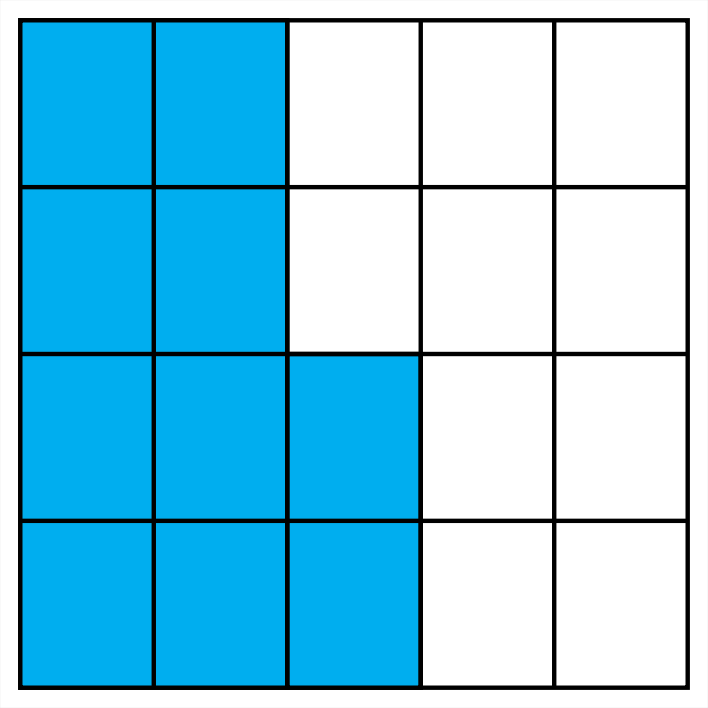
\includegraphics[width=60px]{../images/imagen_frac01.png} \fillin[\fbox{$\dfrac{10}{20}$}][0in] \\[1em]
				\part 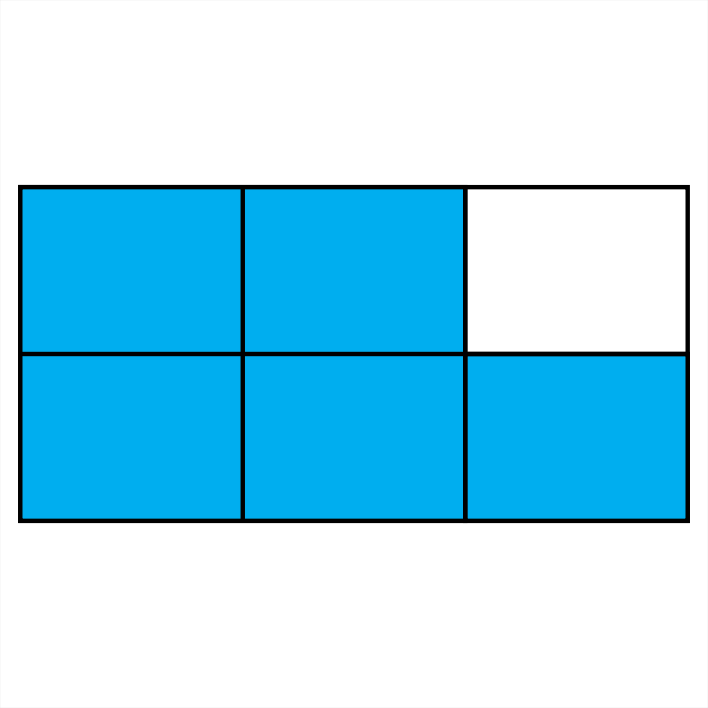
\includegraphics[width=60px]{../images/imagen_frac02.png} \fillin[\fbox{$\dfrac{5}{6}$}][0in] \\[1em]
				\part 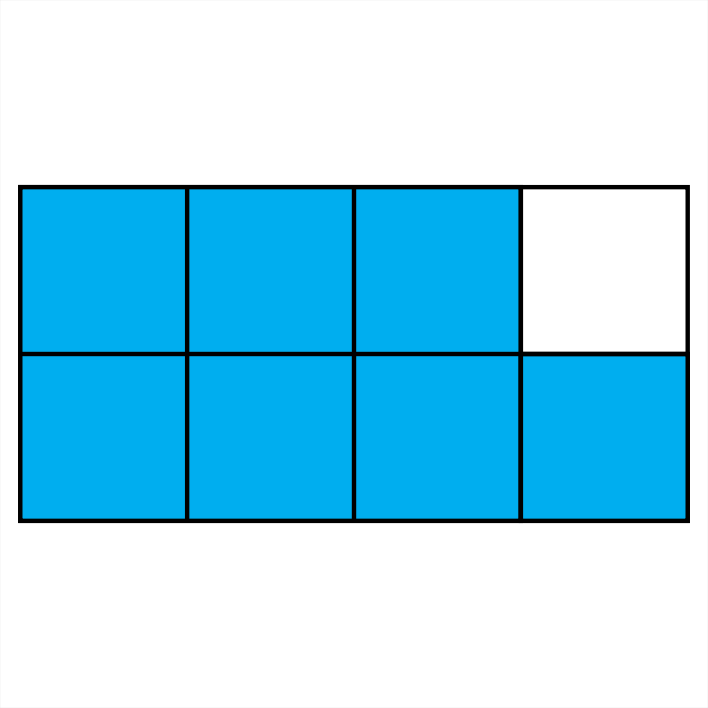
\includegraphics[width=60px]{../images/imagen_frac08.png} \fillin[\fbox{$\dfrac{7}{8}$}][0in] \\[1em]
				\part 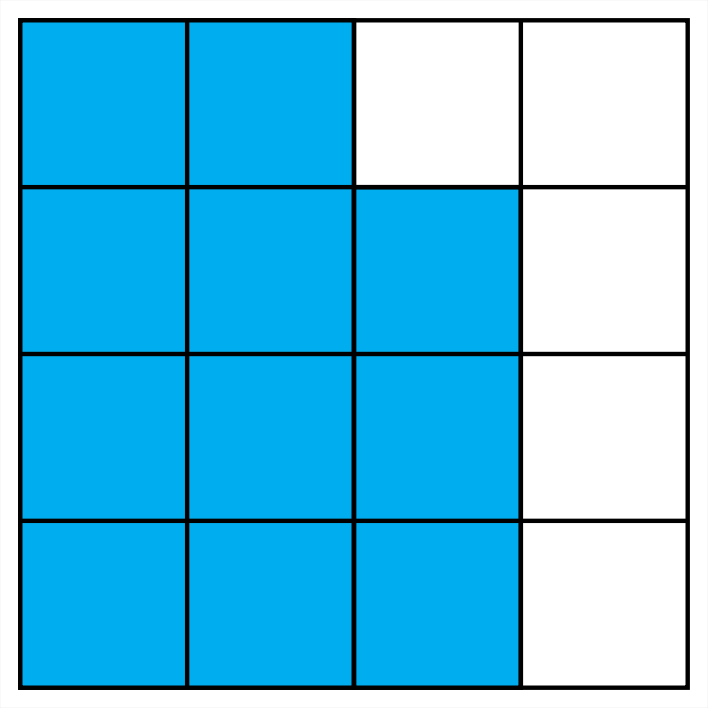
\includegraphics[width=60px]{../images/imagen_frac03.png} \fillin[\fbox{$\dfrac{11}{16}$}][0in] \\[1em]
				% \part 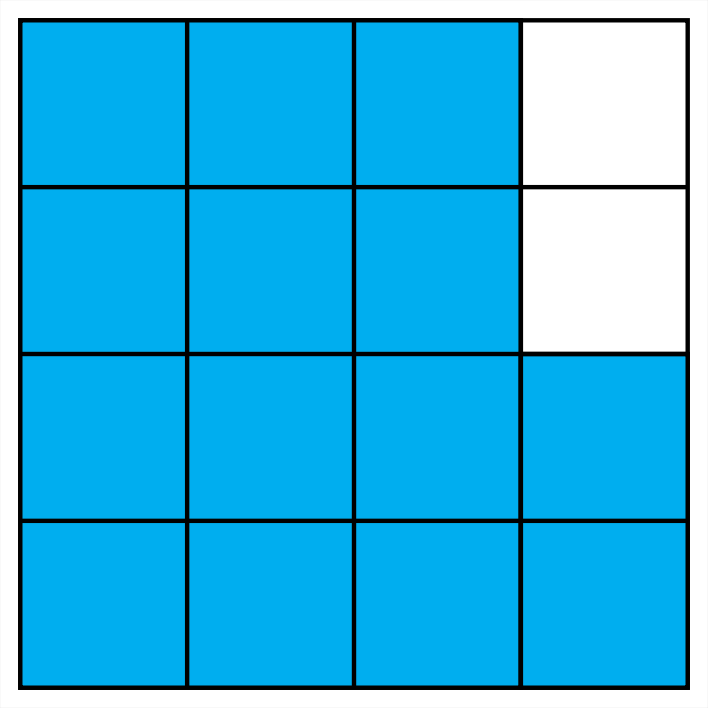
\includegraphics[width=60px]{../images/imagen_frac04.png} \fillin[\fbox{$\dfrac{14}{16}$}][0in] \\[1em]
				\part 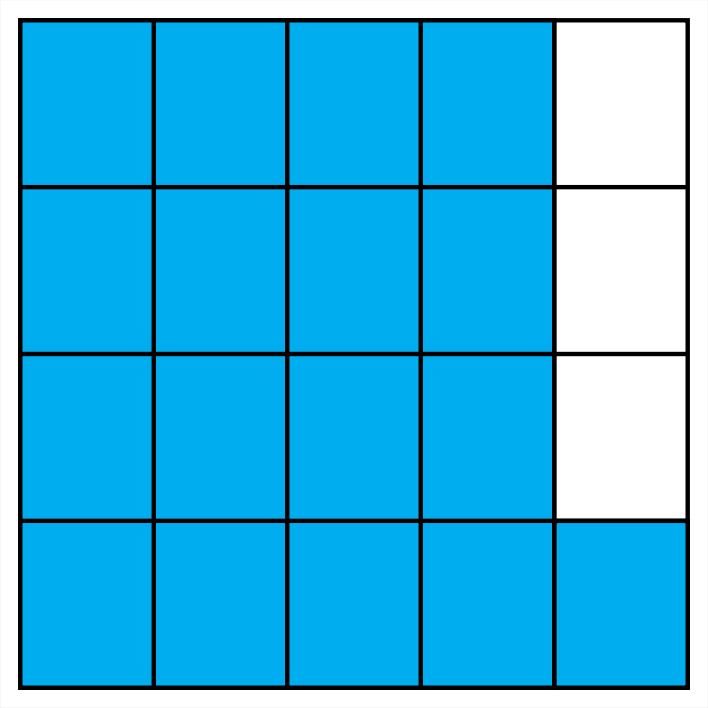
\includegraphics[width=60px]{../images/imagen_frac05.png} \fillin[\fbox{$\dfrac{17}{20}$}][0in] \\[1em]
				\part 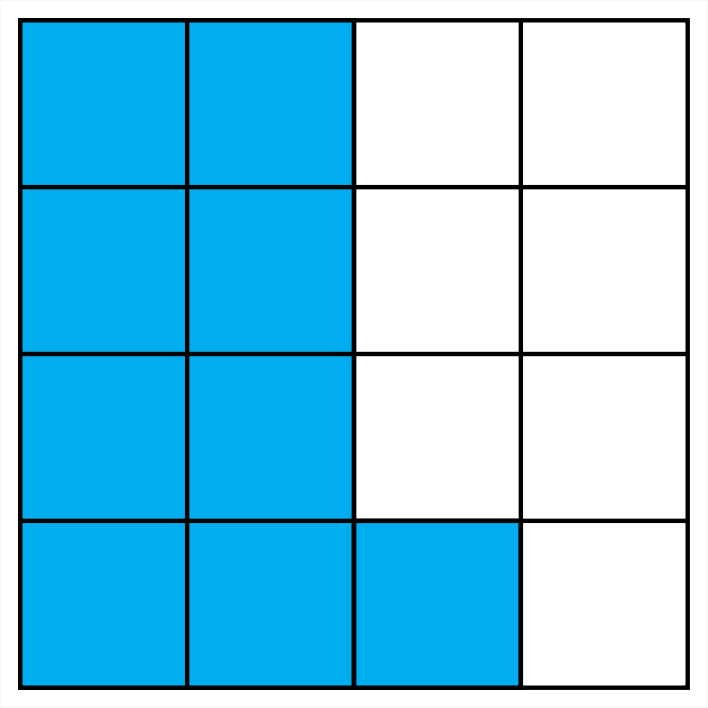
\includegraphics[width=60px]{../images/imagen_frac06.png} \fillin[\fbox{$\dfrac{9}{16}$}][0in] \\[1em]
				% \part 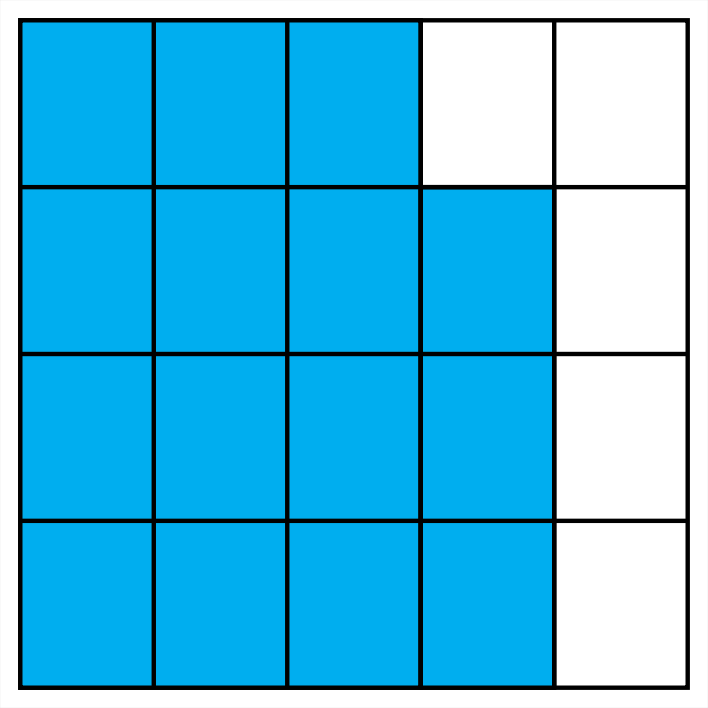
\includegraphics[width=60px]{../images/imagen_frac07.png} \fillin[\fbox{$\dfrac{15}{20}$}][0in] \\[1em]
				% \part 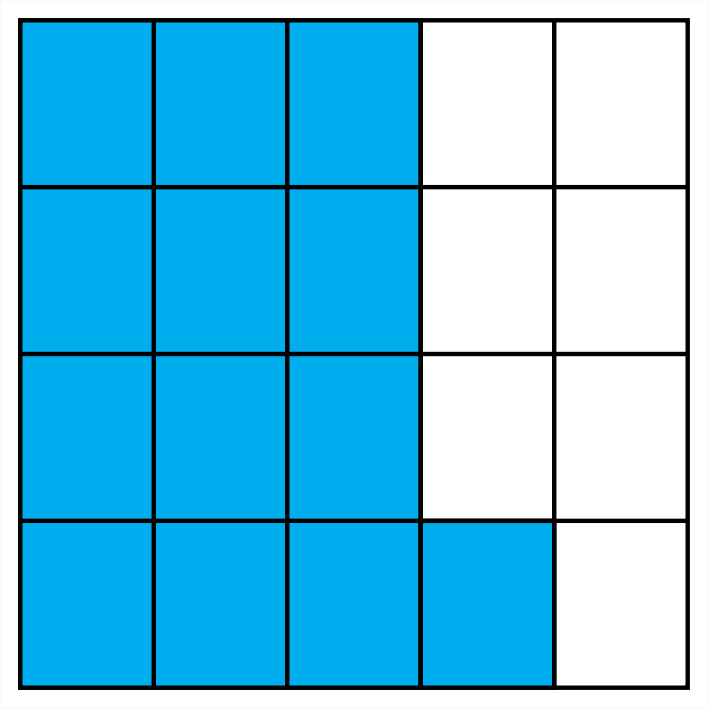
\includegraphics[width=60px]{../images/imagen_frac09.png} \fillin[\fbox{$\dfrac{13}{20}$}][0in] \\[1em]
				\part 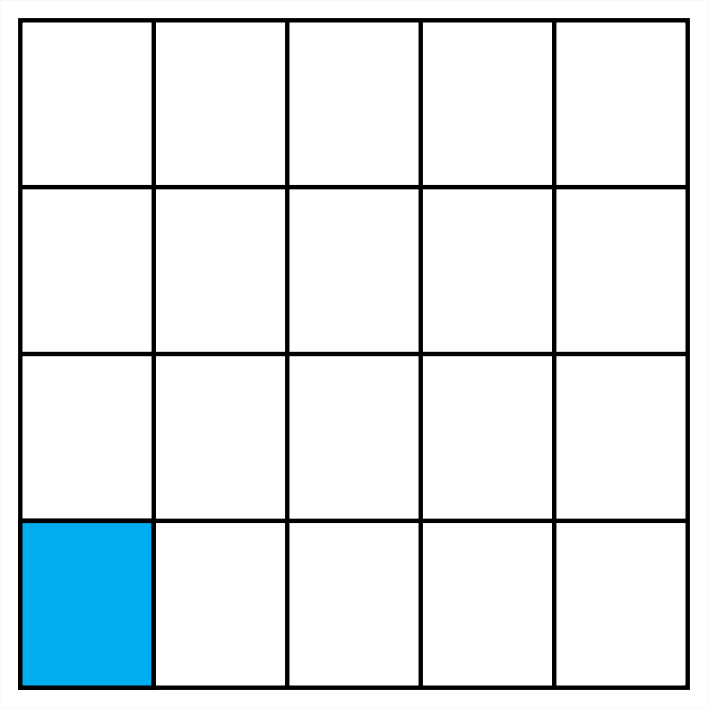
\includegraphics[width=60px]{../images/imagen_frac11.png} \fillin[\fbox{$\dfrac{1}{20}$}][0in] \\[1em]
			\end{parts}
		\end{multicols}
	}

	% \subsection*{\ifprintanswers{Conversión de fracciones mixtas a impropias}\else{}\fi}
	\question[4]{Convierte la siguientes fracciones mixtas a impropias:

		\begin{multicols}{3}
			\begin{parts}
				\part $4\dfrac{2}{3}= $ \fillin[$\dfrac{14}{3}$][0in]
				\part $2\dfrac{3}{10}= $ \fillin[$\dfrac{23}{10}$][0in]
				\part $5\dfrac{1}{5}= $ \fillin[$\dfrac{26}{5}$][0in]
			\end{parts}
		\end{multicols}
	}

	% \subsection*{\ifprintanswers{Conversión de fracciones impropias a mixtas}\else{}\fi}

	\question[4]{Convierte la siguientes fracciones impropias a mixtas:

		\begin{multicols}{3}
			\begin{parts}
				\part $\dfrac{13}{3}= $ \fillin[$4\dfrac{1}{3}$][0in]
				\part $\dfrac{63}{10}= $ \fillin[$6\dfrac{3}{10}$][0in]
				\part $\dfrac{51}{5}= $ \fillin[$10\dfrac{1}{5}$][0in]
			\end{parts}
		\end{multicols}
	}

	\newpage
	\addcontentsline{toc}{subsection}{Operaciones con fracciones}
	\subsection*{Operaciones con fracciones}


	\question[15]{Realiza las siguientes operaciones.

		\begin{multicols}{3}
			\begin{parts}
				\part $\dfrac{5}{4}+\dfrac{1}{4}=$ \fillin[$\dfrac{6}{4}=\dfrac{3}{2}=1\dfrac{1}{2}$][0in] \\[1em]
				\part $1\dfrac{7}{8}-1\dfrac{1}{8}=$ \fillin[$\dfrac{6}{8} = \dfrac{3}{4} $][0in] \\[1em]
				\part $\dfrac{3}{8}+\dfrac{7}{10}=$ \fillin[$\dfrac{43}{40} = 1\dfrac{3}{40}$][0in] \\[1em]
				\part $\dfrac{3}{4}-\dfrac{2}{5}=$ \fillin[$\dfrac{7}{20}$][0in] \\[1em]
				\part $1\dfrac{1}{8}+1\dfrac{7}{8}=$ \fillin[$2\dfrac{8}{8} = 3$][0in] \\[1em]
				\part $\dfrac{3}{10}+\dfrac{4}{5}=$ \fillin[$\dfrac{11}{10} = 1\dfrac{1}{10}$][0in] \\[1em]
				\part $\dfrac{2}{3}-\dfrac{2}{5}=$ \fillin[$\dfrac{4}{15}$][0in] \\[1em]
				\part $\dfrac{3}{5}\times\dfrac{2}{3}=$ \fillin[$\dfrac{6}{15}$][0in]   \\[1em]
				\part $\dfrac{9}{7}-\dfrac{3}{7}=$ \fillin[$\dfrac{6}{7}$][0in] \\[1em]
				\part $\dfrac{7}{8}\times\dfrac{3}{4}=$ \fillin[$\dfrac{21}{32}$][0in] \\[1em]
				\part $\dfrac{3}{5} \divisionsymbol\dfrac{2}{3}=$ \fillin[$\dfrac{9}{10}$][0in] \\[1em]
				\part $\dfrac{7}{8} \divisionsymbol\dfrac{3}{4}=$ \fillin[$\dfrac{28}{24}$][0in]	\\[1em]
			\end{parts}
		\end{multicols}
	}

	\addcontentsline{toc}{subsection}{Figuras geométricas}
	\subsection*{Figuras geométricas}

	\question[2]{Escribe sobre la línea el nombre que recibe cada figura geométrica de acuerdo con su número de lados:

		\begin{multicols}{3}
			\begin{parts}
				\part 
\includegraphics[width=75px]{../images/pentagono_azul.png}  \fillin[pentágono][0.75in]
				\part 
\includegraphics[width=75px]{../images/nonagono_azul.png}   \fillin[nonágono][0.75in]
				\part 
\includegraphics[width=75px]{../images/decagono_azul.png}   \fillin[decágono][0.75in]
				\part 
\includegraphics[width=75px]{../images/hexagono_azul.png}   \fillin[hexágono][0.75in]
				\part 
\includegraphics[width=75px]{../images/rectangulo_azul.png} \fillin[rectángulo][0.75in]
				\part 
\includegraphics[width=75px]{../images/cuadrado_azul.png}   \fillin[cuadrado][0.75in]
			\end{parts}
		\end{multicols}
	}

	% \subsection*{\ifprintanswers{Área de figuras                            }\else{}\fi}

	\question[4]{Contesta las preguntas sobre áreas de figuras geométricas

		\begin{multicols}{2}
			\begin{parts}
				\part ¿Cuál es el área de un triángulo cuya base mide 18 y su altura mide 11?

				\begin{solutionbox}{1.8cm}
					\[A=\dfrac{18 \times 11}{2}=\color{red}99\]
				\end{solutionbox}

				\part ¿Cuál es el área de un cuadrado que sus lados miden 29?

				\begin{solutionbox}{1.8cm}
					\[A=29 \times 29=\color{red}841\]
				\end{solutionbox}
			\end{parts}
		\end{multicols}
	}

	% \subsection*{\ifprintanswers{Perímetros 1                               }\else{}\fi}
	% \subsection*{\ifprintanswers{Perímetros 2                               }\else{}\fi}

	\question[4]{Contesta las preguntas sobre perímetros de figuras geométricas

		\begin{multicols}{2}
			\begin{parts}
				\part ¿Cuál es el perímetro de un rectángulo cuya base mide 38 y su altura mide 19?

				\begin{solutionbox}{1.5cm}
					\[P=38+19+38+19=\color{red}114\]
				\end{solutionbox}

				\part ¿Cuál es el perímetro de un cuadrado que sus lados miden 5?

				\begin{solutionbox}{1.5cm}
					\[P=5+5+5+5=\color{red}20\]
				\end{solutionbox}

				\part ¿Cuál es el perímetro de un pentágono que sus lados miden 18?

				\begin{solutionbox}{1.5cm}
					\[P=18 \times 5=\color{red}90\]
				\end{solutionbox}

				% \part ¿Cuál es el perímetro de un octágono que sus lados miden 15?

				% \begin{solutionbox}{1cm}
				% 	\[P=15 \times 8=\color{red}120\]
				% \end{solutionbox}

				\part ¿Cuál es el perímetro de un rombo que sus lados miden 16?

				\begin{solutionbox}{1.5cm}
					\[P=16 \times 4=\color{red}64\]
				\end{solutionbox}

			\end{parts}
		\end{multicols}
	}


	\addcontentsline{toc}{subsection}{Sistema de unidades}
	\subsection*{Sistema de unidades}

	\question[3]{Realiza las siguientes operaciones:

		\begin{multicols}{3}
			\begin{parts}\large
				\part $ 55 \times 10000=$   \fillin[550000][0.5in]
				\part $ 135 \times 100=$   \fillin[13500][0.5in]
				% \part $ 369 \times 10000=$   \fillin[3690000][0.5in]
				% \part $ 88 \times 10=$   \fillin[880][0.5in]
				% \part $ 1215 \times 100=$   \fillin[121500][0.5in]
				% \part $ 300 \times 10000=$   \fillin[3000000][0.5in]
				\part $ 224 \times 1000=$   \fillin[224000][0.5in]
				\part $ 13 \times 1000=$   \fillin[13000][0.5in]
				% \part $ 134 \times 100000=$   \fillin[13400000][0.5in]
				\part $ 188 \times 10=$   \fillin[1880][0.5in]
				% \part $ 401 \times 1000=$   \fillin[401000][0.5in]
				\part $ 42 \times 10=$   \fillin[420][0.5in]
				\part $ 92 \times 1000=$   \fillin[92000][0.5in]
				\part $ 1050 \times 1000=$   \fillin[1050000][0.5in]
				\part $ 19 \times 100=$   \fillin[1900][0.5in]
			\end{parts}
		\end{multicols}
	}



	% \subsection*{\ifprintanswers{Unidades de tiempo                         }\else{}\fi}
	% \subsection*{\ifprintanswers{Unidades de longitud                       }\else{}\fi}

	\question[3]{Realiza las siguientes conversiones de unidades de longitud:

		\begin{multicols}{2}
			\begin{parts}
				\part De 157 kilómetros a hectómetros. \\ \fillin[1570][0.6in] hm
				\part De 25 centímetros a milímetros.  \\ \fillin[250][0.6in] mm
				% \part De 27 kilómetros a decámetros.   \\ \fillin[2700][0.6in] Dm
				% \part De 17 kilómetros a hectómetros.  \\ \fillin[170][0.6in] hm
				% \part De 69 kilómetros a centímetros.  \\ \fillin[6900000][0.6in] cm
				\part De 59 decímetros a centímetros.  \\ \fillin[590][0.6in] cm
				\part De 26 metros a decímetros.       \\ \fillin[260][0.6in] dm
				\part De 4 kilómetros a milímetros.    \\ \fillin[4000000][0.6in] mm
				\part De 135 kilómetros a decámetros.  \\ \fillin[13500][0.6in] Dm
				% \part De 112 kilómetros a hectómetros. \\ \fillin[1120][0.6in] hm
			\end{parts}
		\end{multicols}
	}


	% \subsection*{\ifprintanswers{Unidades de masa 	                          }\else{}\fi}
	\question[3]{Realiza las siguientes conversiones de unidades de longitud:

		\begin{multicols}{2}
			\begin{parts}
				\part De 205 gramos a decigramos    \hfill \fillin[2050][0.4in] dg
				% \part De 25 kilogramos a gramos     \hfill \fillin[25000][0.5in] g
				\part De 58 kilogramos a gramos     \hfill \fillin[58000][0.4in] g
				\part De 45 decagramos a gramos     \hfill \fillin[450][0.4in] g
				% \part De 134 gramos a decigramos    \hfill \fillin[1340][0.5in] dg
				% \part De 282 gramos a miligramos    \hfill \fillin[282000][0.5in] mg
				\part De 117 decagramos a gramos    \hfill \fillin[1170][0.4in] g
				\part De 17 decigramos a miligramos \hfill \fillin[1700][0.4in] mg
				% \part De 115 gramos a centigramos   \hfill \fillin[11500][0.5in] cg
				\part De 62 gramos a miligramos     \hfill \fillin[62000][0.4in] mg
			\end{parts}
		\end{multicols}
	}
\end{questions}
\end{document}